\documentclass[a4paper, 12pt]{report}
\usepackage{graphicx}
\usepackage[french]{babel}
\usepackage[utf8]{inputenc}
\usepackage[T1]{fontenc}
\usepackage{multirow}
\usepackage{listings}
\usepackage{float}
\usepackage[french]{babel}
\usepackage[breaklinks]{hyperref}
\hypersetup{pageanchor=false}

\begin{document}

\begin{titlepage}
  \begin{center}
    \begin{tabular*}{\textwidth}{l@{\extracolsep{\fill}}r}
      
\includegraphics[height=1.5cm]{images/m1info.png}&
			
\includegraphics[height=1.5cm]{images/P8.png}
    \end{tabular*}
    \small 
    \rule{\textwidth}{.5pt}~\\
    \large 
    \textsc{Université Paris 8 - Vincennes à Saint-Denis}\vspace{0.5cm}\\
    \textbf{Master Informatique des Systèmes Embarqués}\vspace{3.0cm}\\
    \Large
    \textbf{Rapport de projet tuteuré}\vspace{1.5cm}\\
    \large
    \textbf{Samuel \textsc{de Vals}}\\
		\textbf{Paul \textsc{Vialart}}\vspace{1.5cm}\\
    Date de soutenance : le 19/01/2018\vspace{1.75cm}\\
  \end{center}\vspace{1.5cm}~\\
  \begin{tabular}{ll}
    \hspace{-0.45cm}Tuteur -- Université~:~&~Sylvia \textsc{Chalençon}
  \end{tabular}
\end{titlepage}

\newpage\null\newpage

\chapter*{Résumé}
\markboth{\sc Résumé}{}
\addcontentsline{toc}{chapter}{Résumé} 
L'intérêt de ce projet est la reproduction d'une carte en trois dimensions générée avec le "`bruit de Perlin"'. Ce sujet nous a été attribué en raison de la variété d'aspects techniques qu'il permet de traiter : les rendus en 3D en temps réel, bien sûr, mais aussi l'aspect visuel et graphique ; la partie fonctionnelle (dans le sens où l'utilisateur doit pouvoir effectuer une liste d'actions, qu'il nous revient de gérer à l'intérieur du programme) ; et enfin, et non des moindres, la partie algorithmique (ce point précis sera développé plus en aval au cours de ce document).
En effet, le  Bruit de Perlin permet la génération de matrices de manière procédurale : ainsi, le rendu visuel est différent à chaque lancement du programme. Le bruit de Perlin fait partie des algorithmes les plus célèbres de certaines industries, comme le jeu vidéo. Le but est donc de pouvoir reproduire ce processus, avec la particularité d'un habillage en "`style Lego"'.

Pour le moment, nous avons reconstitué l'algorithme du bruit de Perlin en Javascript, et nous l'avons intégré à un module three.JS afin de reproduire un monde cubique en 3D.


\chapter*{Introduction}
\markboth{\sc Introduction}{}
\addcontentsline{toc}{chapter}{Introduction}
\input{teX/001_introduction.tex}

%adding content into the summary page /!\ need 2 compilations
\tableofcontents

\chapter*{Le choix de l'API three.JS}
\markboth{\sc Le choix de l'API three.JS}{}
\addcontentsline{toc}{chapter}{Le choix de l'API three.JS}
Nous avons tout d'abord découpé le projet en différentes tâches à réaliser afin de le mener à son terme. Voici un schéma représentant les principales étapes d'élaboration du projet.

\begin{center}
	\includegraphics[height=7cm]{images/Processus_DEV.png}\\
	\textit{Processus de développement utilisé au cours du projet}\\
\end{center}

\newpage
Nous avons choisi l'API three.JS car celle-ci permet de faire du WebGL de façon simple et facilite la mise en œuvre du projet. En effet, ce projet est notre premier contact avec le domaine du WebGL. De plus, nous avons repris le code d'un exemple de cette API.Cet exemple génère un monde virtuel avec le bruit de Perlin, qui rappelle le jeu vidéo Minecraft. Voici le rendu graphique de l'exemple :

\begin{center}
	\includegraphics[height=6cm]{images/threeJS_minecraft.png}\\
	\textit{Exemple du monde virtuel généré avec l'API three.JS}
	\footnote{Le code source de l'exemple de l'API three.JS se trouve là : \url{https://github.com/mrdoob/three.js/blob/master/examples/webgl_geometry_minecraft.html}}
\end{center}

Il a ensuite fallu adapter le projet afin de mettre le code source HTML, CSS, et JS dans des fichiers séparés.

\begin{center}
	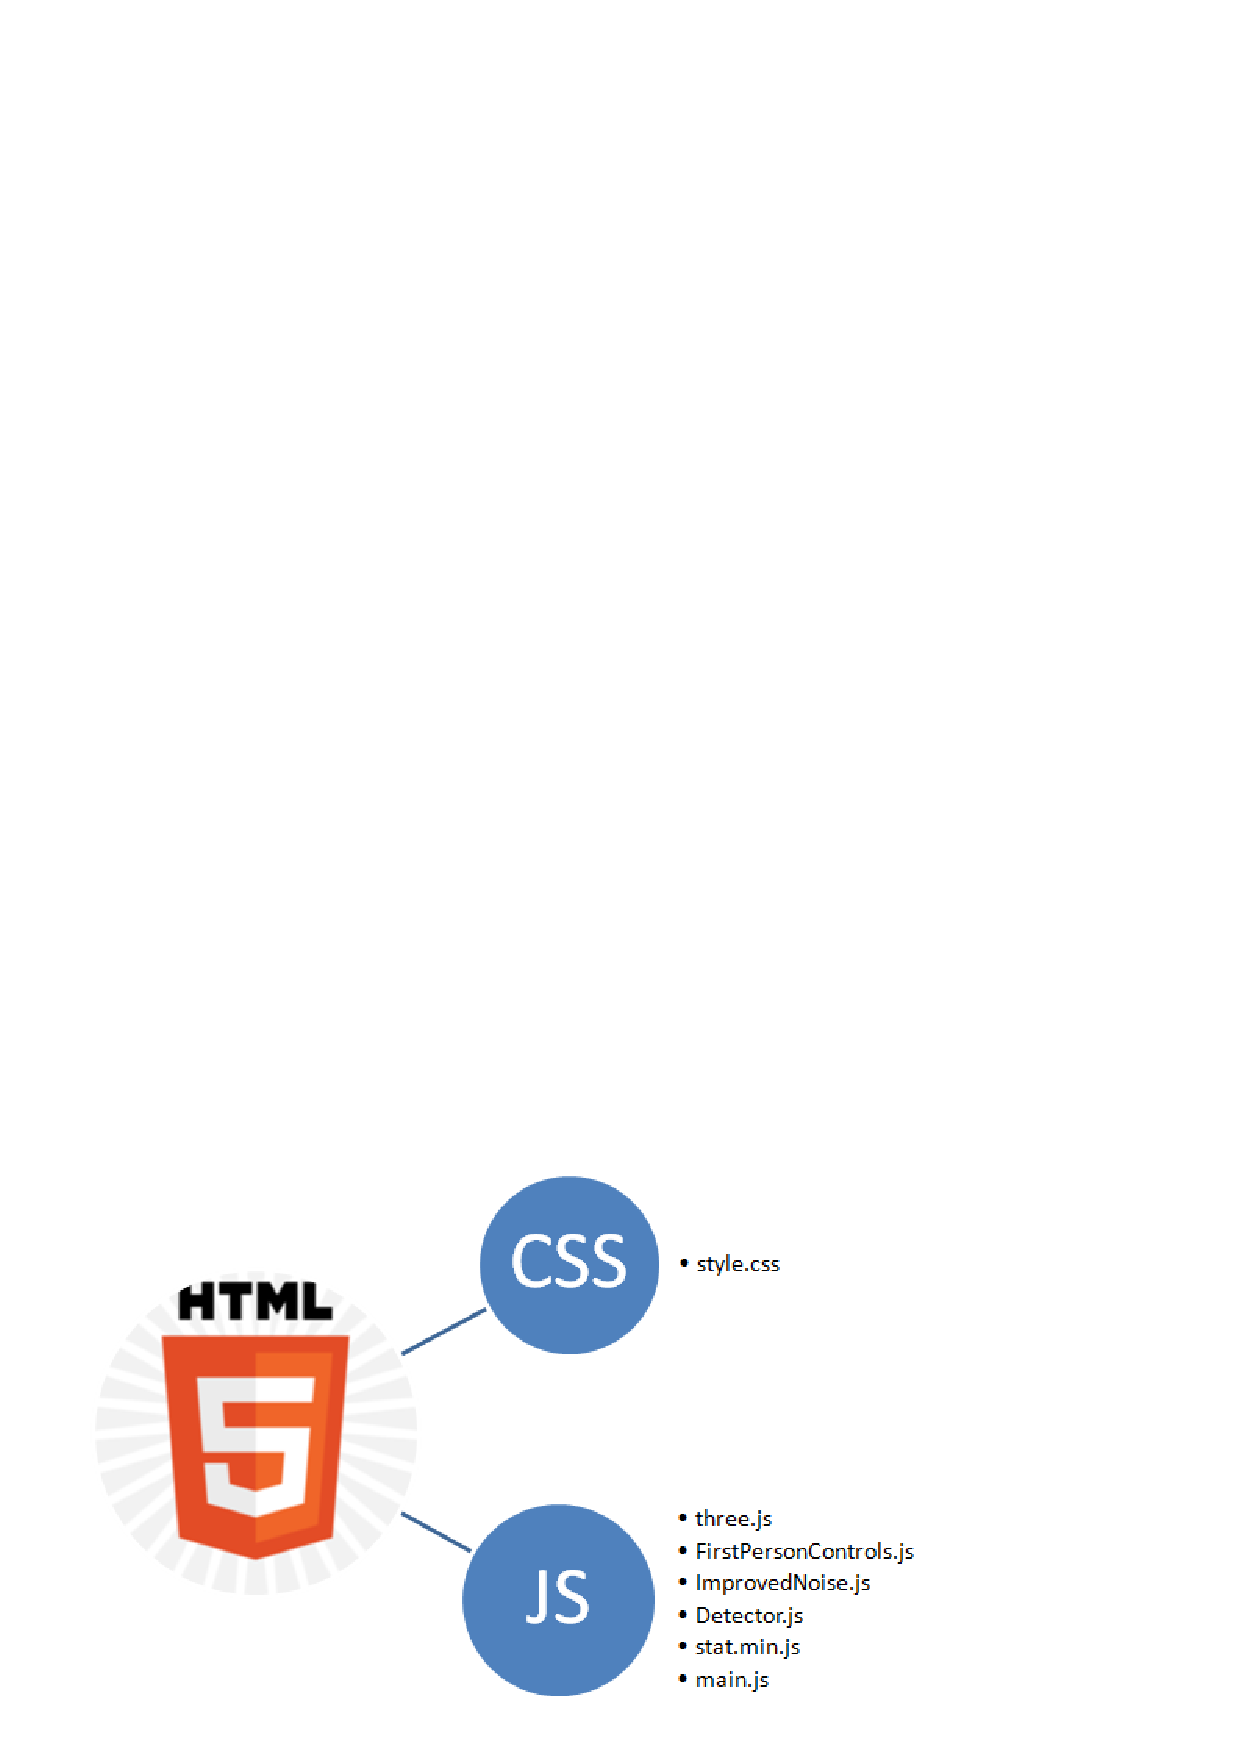
\includegraphics[height=6cm]{images/ProFileOrganisation.png}\\
	\textit{Structure du projet}
\end{center}

\chapter*{Le bruit de Perlin}
\markboth{\sc Le bruit de Perlin}{}
\addcontentsline{toc}{chapter}{Le bruit de Perlin}
Le \textbf{bruit de Perlin} est très utilisé dans la génération d'image. Développé par Ken Perlin en 1985, il a depuis largement été repris par toutes sortes d'industries afin de générer, entre autres, des rendus topographiques.	Il permet en effet de remplir une matrice de N dimensions (dans notre cas 3), ce qui se traduit par une élévation de sommets et un rendu graphique cohérent. Nous avons donc implémenté un algorithme de afin de générer ce bruit de Perlin. 

L'algorithme se divise en deux temps :

\begin{enumerate}
	\item Initialisation
	\item Calcul
\end{enumerate}

La phase d'initialisation consite à avoir un tableau de 512 éléments bien mélangés compris entre 0 et 255. Ensuite, le tableau se répète à partir de la valeur 256 (tab[0] = tab[256], et ainsi de suite). 

La phase de calcul est plus compliquée, car elle se découpe en plusieurs étapes. Le principe de l'algorithme est de retourner une même valeur en fonction d'un x, d'un y, et d'un z donné. On place x, y , z dans l'intervalle [0;255] avec un "et" logique. Ensuite on calcule les coordonnées en gradient du cube dans l'espace. Enfin, on calcule la valeur de retour. 

Afin de générer aléatoirement un monde virtuel, il est necessaire de remplir le tableau aléatoirement à chaque démarrage du projet. Sinon on obtiendra toujours la même monde carte, car le tableau de permutation reste toujours le même entre deux chargements.

A noter que Ken Perlin a ensuite amélioré cet algorithme, afin qu'il soit plus performant en terme de calcul et de résultat. Publiée en 2001, cette version s'appelle le bruit de Simplex.


\chapter*{Les axes d'améliorations}
\markboth{\sc Les axes d'améliorations}{}
\addcontentsline{toc}{chapter}{Les axes d'améliorations}
Nous avons réfléchis a différents axes d'améliorations, que nous implémenterons si nous avons le temps. Voici une liste des améliorations par ordre de priorité :

\vspace{0.5cm}
\begin{enumerate}
	\item Améliorer la structure du code
	\item Changer les textures en fonction de l'altitude
	\item Utiliser les flèches directionnelles pour se déplacer
	\item Se déplacer dans le monde sans traverser les blocs
	\item Implémenter génération de terrain avec le bruit de simplex
	\item Ajouter divers éléments de décors (arbes, cours d'eau, etc.)
\end{enumerate}
\vspace{0.5cm}









\chapter*{Conclusion}
\markboth{\sc Conclusion}{}
\addcontentsline{toc}{chapter}{Conclusion}
La découverte des technologies tel que le webGL, et la rédaction de document en lateX a été très enrichissante. En effet, nous avons pu rapidement voir ce qu'il était possible de faire en webGL à travers l' API three.JS qui propose un large panel d'exemple. De plus, nous avons pu étudier le fonctionnement de l'algorithme de génération de bruit de Perlin qui est très utilisé dans le monde de génération procédurale de terrain. Cependant, il nous reste encore beaucoup à faire pour terminer ce projet.



\chapter*{Bibliographie}
\markboth{\sc Bibliographie}{}
\addcontentsline{toc}{chapter}{Bibliographie}
\input{teX/006_Bibliographie.tex}

\end{document}